\section{Historical Development of Neural Networks}

\subsection{Timeline of Neural Network Evolution}
The development of neural networks has proceeded through several distinct phases, each marked by significant theoretical breakthroughs and practical applications.

\begin{table}[h!]
\centering
\small
\begin{tabular}{|p{1.5cm}|p{1cm}|p{3.5cm}|p{2.5cm}|p{5cm}|}
\hline
\textbf{Period} & \textbf{Year} & \textbf{Key Development} & \textbf{Contributors} & \textbf{Description} \\
\hline
\textbf{Early Foundations} & 1943 & McCulloch-Pitts Neuron & Warren McCulloch, Walter Pitts & First mathematical model of artificial neuron using threshold logic \\
\hline
& 1949 & Hebbian Learning Rule & Donald Hebb & "Cells that fire together, wire together" - synaptic plasticity principle \\
\hline
\textbf{First Generation} & 1957 & Perceptron & Frank Rosenblatt & First trainable neural network with learning algorithm \\
\hline
& 1960 & ADALINE/MADALINE & Bernard Widrow, Marcian Hoff & Adaptive linear neurons with delta rule learning \\
\hline
\textbf{Winter Period} & 1969 & Perceptron Limitations & Marvin Minsky, Seymour Papert & Proved perceptrons cannot solve XOR problem \\
\hline
\textbf{Revival Era} & 1982 & Hopfield Networks & John Hopfield & Recurrent networks for associative memory \\
\hline
& 1986 & Backpropagation & Rumelhart, Hinton, Williams & Efficient algorithm for training multi-layer networks \\
\hline
\textbf{Modern Era} & 2012 & AlexNet & Alex Krizhevsky, Geoffrey Hinton & Deep CNN wins ImageNet competition \\
\hline
& 2017 & Transformer Architecture & Vaswani et al. (Google) & Attention-based model for sequences \\
\hline
\end{tabular}
\caption{Key milestones in neural network development.}
\end{table}

\subsection{Threshold Logic: The Foundation}
The simplest kind of computing units used to build artificial neural networks are based on threshold logic. These computing elements are a generalization of the common logic gates used in conventional computing and, since they operate by comparing their total input with a threshold, this field of research is known as \textbf{threshold logic}.

\section{McCulloch-Pitts Neuron: The First Artificial Neuron}
The McCulloch-Pitts neuron, introduced in 1943, was the first mathematical model of an artificial neuron. It established the theoretical foundation for neural computation using threshold logic.

\subsection{Mathematical Model}
The McCulloch-Pitts neuron computes its output according to:
\[
y = \begin{cases}
 1 & \text{if } \displaystyle\sum_{i=1}^{n} w_i x_i \geq \theta \\
 0 & \text{otherwise}
\end{cases}
\]

Where:
\begin{itemize}
    \item $x_i$ are the input values (binary: 0 or 1)
    \item $w_i$ are the corresponding weights
    \item $\theta$ is the threshold value
    \item $y$ is the binary output (0 or 1)
\end{itemize}

\subsection{Logic Gate Implementation}
The McCulloch-Pitts model can implement basic logic functions:

\subsubsection{AND Gate}
For an AND gate with two inputs:
\begin{itemize}
    \item Weights: $w_1 = w_2 = 1$
    \item Threshold: $\theta = 2$
    \item Result: Output is 1 only when both inputs are 1
\end{itemize}

\subsubsection{OR Gate}
For an OR gate with two inputs:
\begin{itemize}
    \item Weights: $w_1 = w_2 = 1$
    \item Threshold: $\theta = 1$
    \item Result: Output is 1 when at least one input is 1
\end{itemize}

\subsection{Limitations of McCulloch-Pitts Neurons}
\begin{itemize}
    \item \textbf{Fixed weights}: No learning mechanism
    \item \textbf{Binary inputs only}: Cannot handle continuous values
    \item \textbf{Synchronous operation}: All neurons fire simultaneously
    \item \textbf{No adaptation}: Cannot modify behavior based on experience
\end{itemize}

These limitations led to the development of the Perceptron, which introduced learning capabilities.

\section{The Perceptron: A Detailed Introduction}
The Perceptron is a simple binary classifier that serves as the foundational building block for more complex neural networks.

\subsection{Definition: The Anatomy of a Perceptron}
For an input vector \(\mathbf{x} = (x_1, x_2, \dots, x_n)\), the Perceptron computes a single output \(y\). This is done in two steps:
\begin{enumerate}
    \item \textbf{Compute a Weighted Sum:} The model calculates a weighted sum of the inputs, adding a bias. This is the net input \(z\).
    \[ z = (w_1 x_1 + w_2 x_2 + \dots + w_n x_n) + b = \mathbf{w} \cdot \mathbf{x} + b \]
    \item \textbf{Apply an Activation Function:} The output \(z\) is passed through a Heaviside step function.
    \[ y = \phi(z) = \begin{cases} 1 & \text{if } z \ge 0 \\ 0 & \text{if } z < 0 \end{cases} \]
\end{enumerate}

\section{The Perceptron Learning Rule}
The Perceptron learns by adjusting its weights \(\mathbf{w}\) and bias \(b\) based on the errors it makes. This learning rule has strong theoretical foundations.

\subsection{Mathematical Derivation}
For a given training example \((\mathbf{x}, t)\), where \(t\) is the true target label, the error \(\epsilon\) is calculated as \(\epsilon = t - y\). The weights and bias are then updated:
\[ w_i(\text{new}) = w_i(\text{old}) + \eta \cdot \epsilon \cdot x_i \]
\[ b(\text{new}) = b(\text{old}) + \eta \cdot \epsilon \]
Where \(\eta\) is the learning rate.

\subsection{Convergence Theorem (Rosenblatt, 1962)}
\textbf{Theorem}: If the training data is linearly separable, the perceptron learning algorithm will converge to a solution in a finite number of steps.

\subsubsection{Proof Sketch}
Let \(\mathbf{w}^*\) be a weight vector that correctly classifies all training examples with margin \(\gamma > 0\):
\[y_i(\mathbf{w}^{*T} \mathbf{x}_i) \geq \gamma \quad \forall i\]

The proof shows that:
\begin{enumerate}
    \item The dot product \(\mathbf{w}_t \cdot \mathbf{w}^*\) grows linearly with updates
    \item The norm \(||\mathbf{w}_t||^2\) grows at most linearly with updates
    \item This leads to a contradiction if the algorithm doesn't converge
\end{enumerate}

\subsubsection{Convergence Bound}
The perceptron will make at most \(\left(\frac{R}{\gamma}\right)^2\) mistakes, where:
\begin{itemize}
    \item \(R\) is the maximum norm of any training example: \(R = \max_i ||\mathbf{x}_i||\)
    \item \(\gamma\) is the margin of the optimal separating hyperplane
\end{itemize}

\subsection{Learning Rate Analysis}
\subsubsection{Effect of Learning Rate \(\eta\)}
\begin{itemize}
    \item \textbf{Large \(\eta\)}: Faster convergence but may overshoot optimal solution
    \item \textbf{Small \(\eta\)}: More stable learning but slower convergence
    \item \textbf{Theoretical Result}: For linearly separable data, any \(\eta > 0\) guarantees convergence
\end{itemize}

\subsubsection{Adaptive Learning Rates}
Common strategies include:
\begin{itemize}
    \item \textbf{Time decay}: \(\eta_t = \frac{\eta_0}{1 + \alpha t}\)
    \item \textbf{Step decay}: Reduce \(\eta\) by factor every few epochs
    \item \textbf{Performance-based}: Reduce \(\eta\) when performance plateaus
\end{itemize}

\section{Vectorisation of Perceptron Learning Rule: A Matrix-Based Example}
To see how vectorization works in practice, let's walk through the process using a full matrix-based approach for the AND function. This method calculates the updates for all samples in the dataset (a "batch") and then applies a single, consolidated update at the end of the epoch.

\subsection{Mathematical Foundation of Vectorization}
Vectorization allows us to process multiple training examples simultaneously using matrix operations instead of iterating through samples one by one. This approach is:
\begin{itemize}
    \item \textbf{Computationally efficient}: Modern hardware (GPUs) excels at matrix operations
    \item \textbf{Mathematically elegant}: Compact representation of batch operations
    \item \textbf{Numerically stable}: Reduces accumulated floating-point errors
\end{itemize}

\subsection{Define the Matrices}
For the AND function, we use an augmented Input Matrix \(X\), a Weight Vector \(W\), and a Target Vector \(T\).

\subsubsection{Input Matrix \(X\) (Augmented Design Matrix)}
The input matrix includes a bias column (first column of 1s) followed by the feature columns:
\[
X = \begin{pmatrix}
1 & 0 & 0 \\
1 & 0 & 1 \\
1 & 1 & 0 \\
1 & 1 & 1
\end{pmatrix}_{4 \times 3}
\]
where:
\begin{itemize}
    \item Rows represent training examples (4 samples)
    \item First column represents bias input (always 1)
    \item Remaining columns represent feature inputs \(x_1, x_2\)
\end{itemize}

\subsubsection{Target Vector \(T\)}
\[
T = \begin{pmatrix}
0 \\
0 \\
0 \\
1
\end{pmatrix}_{4 \times 1}
\]

\subsubsection{Weight Vector \(W\)}
Let's initialize the weight vector \(W\) to zeros and use a learning rate \(\eta = 0.1\).
\[
W_0 = \begin{pmatrix}
w_0 \\
w_1 \\
w_2
\end{pmatrix} = \begin{pmatrix}
0 \\
0 \\
0
\end{pmatrix}_{3 \times 1}
\]
where \(w_0\) is the bias weight, \(w_1\) and \(w_2\) are feature weights.

\subsection{Epoch 1: Mathematical Flow}
\subsubsection{Step 1: Compute Net Input Z}
The net input is computed as \(Z = X \cdot W\), where we multiply the \(4 \times 3\) input matrix by the \(3 \times 1\) weight vector to get a \(4 \times 1\) output vector.
\[
Z = X \cdot W_0 = \begin{pmatrix}
1 & 0 & 0 \\
1 & 0 & 1 \\
1 & 1 & 0 \\
1 & 1 & 1
\end{pmatrix}_{4 \times 3} \begin{pmatrix}
0 \\
0 \\
0
\end{pmatrix}_{3 \times 1} = \begin{pmatrix}
1 \cdot 0 + 0 \cdot 0 + 0 \cdot 0 \\
1 \cdot 0 + 0 \cdot 0 + 1 \cdot 0 \\
1 \cdot 0 + 1 \cdot 0 + 0 \cdot 0 \\
1 \cdot 0 + 1 \cdot 0 + 1 \cdot 0
\end{pmatrix} = \begin{pmatrix}
0 \\
0 \\
0 \\
0
\end{pmatrix}_{4 \times 1}
\]

\textbf{Matrix Dimension Check:} \((4 \times 3) \times (3 \times 1) = (4 \times 1)\) 

\subsubsection{Step 2: Apply Activation Function to get Output Y}
Apply the Heaviside step function element-wise: \(\phi(z) = \begin{cases} 1 & \text{if } z \geq 0 \\ 0 & \text{if } z < 0 \end{cases}\)
\[
Y = \phi(Z) = \phi \begin{pmatrix}
0 \\
0 \\
0 \\
0
\end{pmatrix}_{4 \times 1} = \begin{pmatrix}
\phi(0) \\
\phi(0) \\
\phi(0) \\
\phi(0)
\end{pmatrix} = \begin{pmatrix}
1 \\
1 \\
1 \\
1
\end{pmatrix}_{4 \times 1}
\]
Since all net inputs are 0, and \(\phi(0) = 1\) by our step function definition, all outputs are 1.

\subsubsection{Step 3: Calculate the Error Vector E}
\[
E = T - Y =
\begin{pmatrix}
0 \\
0 \\
0 \\
1
\end{pmatrix}
-
\begin{pmatrix}
1 \\
1 \\
1 \\
1
\end{pmatrix}
=
\begin{pmatrix}
-1 \\
-1 \\
-1 \\
0
\end{pmatrix}
\]

\subsubsection{Step 4: Calculate the Total Weight Update \(\Delta W\)}
The weight update is computed as \(\Delta W = \eta \cdot (X^T \cdot E)\), where we multiply the transpose of the input matrix by the error vector.

First, let's compute \(X^T\):
\[
X^T = \begin{pmatrix}
1 & 0 & 0 \\
1 & 0 & 1 \\
1 & 1 & 0 \\
1 & 1 & 1
\end{pmatrix}^T = \begin{pmatrix}
1 & 1 & 1 & 1 \\
0 & 0 & 1 & 1 \\
0 & 1 & 0 & 1
\end{pmatrix}_{3 \times 4}
\]

Now compute the weight update:
\[
\Delta W = \eta \cdot (X^T \cdot E) = 0.1 \cdot \begin{pmatrix}
1 & 1 & 1 & 1 \\
0 & 0 & 1 & 1 \\
0 & 1 & 0 & 1
\end{pmatrix}_{3 \times 4} \begin{pmatrix}
-1 \\
-1 \\
-1 \\
0
\end{pmatrix}_{4 \times 1}
\]

\[
= 0.1 \cdot \begin{pmatrix}
1(-1) + 1(-1) + 1(-1) + 1(0) \\
0(-1) + 0(-1) + 1(-1) + 1(0) \\
0(-1) + 1(-1) + 0(-1) + 1(0)
\end{pmatrix} = 0.1 \cdot \begin{pmatrix}
-3 \\
-1 \\
-1
\end{pmatrix} = \begin{pmatrix}
-0.3 \\
-0.1 \\
-0.1
\end{pmatrix}_{3 \times 1}
\]

\textbf{Matrix Dimension Check:} \((3 \times 4) \times (4 \times 1) = (3 \times 1)\) 

\subsubsection{Step 5: Update the Weight Vector W}
\[
W_1 = W_0 + \Delta W =
\begin{pmatrix}
0 \\
0 \\
0
\end{pmatrix}
+
\begin{pmatrix}
-0.3 \\
-0.1 \\
-0.1
\end{pmatrix}
=
\begin{pmatrix}
-0.3 \\
-0.1 \\
-0.1
\end{pmatrix}
\]
After the first epoch, our new weight vector is \(W_1 = (-0.3, -0.1, -0.1)^T\).

\subsection{Mathematical Insight: Gradient Descent Connection}
The vectorized perceptron learning rule is actually a special case of gradient descent. The weight update \(\Delta W = \eta \cdot X^T \cdot E\) can be derived from minimizing the perceptron loss function:

\subsubsection{Loss Function}
For a single misclassified example, the perceptron loss is:
\[L = \max(0, -y_{\text{true}} \cdot z)\]
where \(z = \mathbf{w}^T \mathbf{x}\) is the net input.

\subsubsection{Gradient of the Loss}
The gradient with respect to weights is:
\[\frac{\partial L}{\partial \mathbf{w}} = -y_{\text{true}} \cdot \mathbf{x}\]
for misclassified examples, and 0 for correctly classified ones.

\subsubsection{Batch Update Rule}
For a batch of examples, the total gradient is:
\[\frac{\partial L_{\text{total}}}{\partial \mathbf{w}} = \sum_{i} \frac{\partial L_i}{\partial \mathbf{w}} = X^T \cdot (Y_{\text{pred}} - Y_{\text{true}})\]

This shows that our vectorized update rule \(\Delta W = \eta \cdot X^T \cdot E\) is exactly gradient descent with the perceptron loss function.

\subsection{Computational Complexity Analysis}
\subsubsection{Vectorized vs. Sequential Processing}
\begin{itemize}
    \item \textbf{Sequential}: \(O(m \cdot n)\) time for \(m\) examples and \(n\) features, but cannot leverage parallel hardware
    \item \textbf{Vectorized}: Same \(O(m \cdot n)\) time complexity, but:
    \begin{itemize}
        \item Can utilize SIMD (Single Instruction, Multiple Data) operations
        \item Reduces Python interpreter overhead
        \item Enables GPU acceleration for large matrices
        \item Better cache locality and memory access patterns
    \end{itemize}
\end{itemize}

\section{Geometric Interpretation of the Perceptron}
Understanding a Perceptron involves grasping the geometry of how it makes decisions. We can visualize this geometry in two primary ways: the \textbf{Input Space} and the \textbf{Weight Space}.

\subsection{Mathematical Foundation of Decision Boundaries}
The perceptron's decision boundary is defined by the hyperplane equation:
\[\mathbf{w}^T \mathbf{x} + b = 0\]

\subsubsection{Hyperplane Properties}
\begin{itemize}
    \item \textbf{Normal Vector}: The weight vector \(\mathbf{w}\) is perpendicular to the decision boundary
    \item \textbf{Distance from Origin}: \(\frac{|b|}{||\mathbf{w}||_2}\) gives the perpendicular distance from the hyperplane to the origin
    \item \textbf{Classification Rule}:
    \begin{itemize}
        \item Points where \(\mathbf{w}^T \mathbf{x} + b > 0\) are classified as positive (class 1)
        \item Points where \(\mathbf{w}^T \mathbf{x} + b < 0\) are classified as negative (class 0)
        \item Points on the boundary satisfy \(\mathbf{w}^T \mathbf{x} + b = 0\)
    \end{itemize}
\end{itemize}

\subsubsection{Margin and Support}
The \textbf{functional margin} of a point \(\mathbf{x}_i\) with true label \(y_i \in \{-1, +1\}\) is:
\[\gamma_i = y_i(\mathbf{w}^T \mathbf{x}_i + b)\]

The \textbf{geometric margin} is the normalized version:
\[\hat{\gamma}_i = \frac{y_i(\mathbf{w}^T \mathbf{x}_i + b)}{||\mathbf{w}||_2}\]

This represents the perpendicular distance from the point to the decision boundary.

\subsection{Example: The NOT Function}
\subsubsection{The Input Space}
The Input Space is a geometric representation of the data points. The goal of the Perceptron is to find a \textbf{decision boundary}---a line in 2D, or a hyperplane in higher dimensions---that perfectly separates the positive and negative data points.
\begin{figure}[h!]
\centering
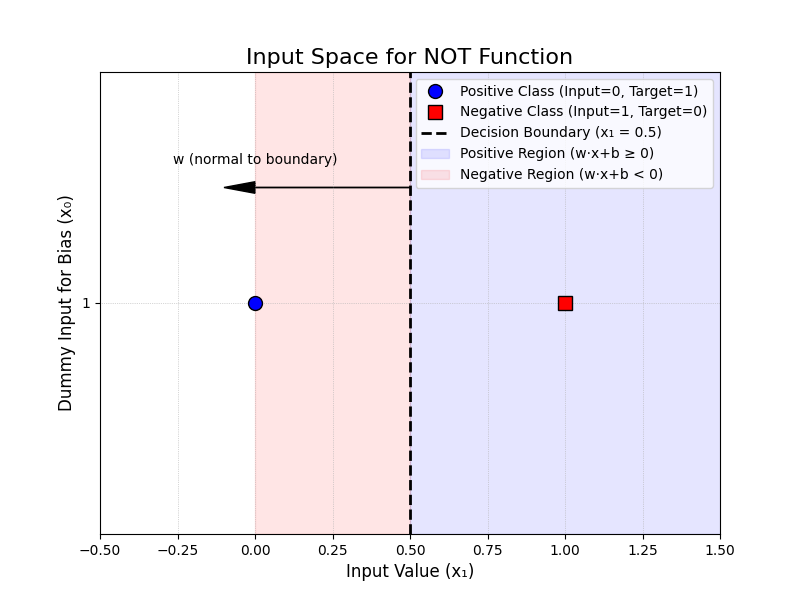
\includegraphics[width=0.6\textwidth]{not_input_space.png}
\caption{Input Space for the NOT Function.}
\end{figure}

\subsubsection{The Weight Space}
While the input space plots the data, the \textbf{Weight Space} plots the possible solutions. The axes of this space are the weights themselves. Every point in this space represents a different Perceptron model.
\begin{figure}[h!]
\centering
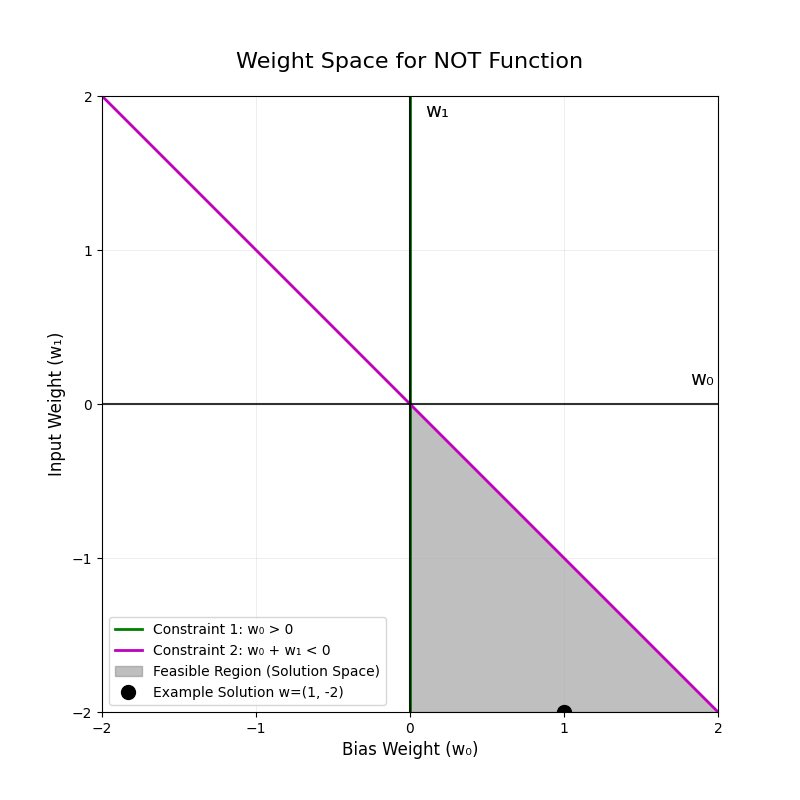
\includegraphics[width=0.6\textwidth]{not_weight_space.png}
\caption{Weight Space for the NOT Function.}
\end{figure}

\subsection{Example: The AND Function}
\subsubsection{The Input Space}
The Input Space shows our data points and the decision boundary that separates them. For the AND function, we have three "negative" points (target=0) and one "positive" point (target=1).
\begin{figure}[h!]
\centering
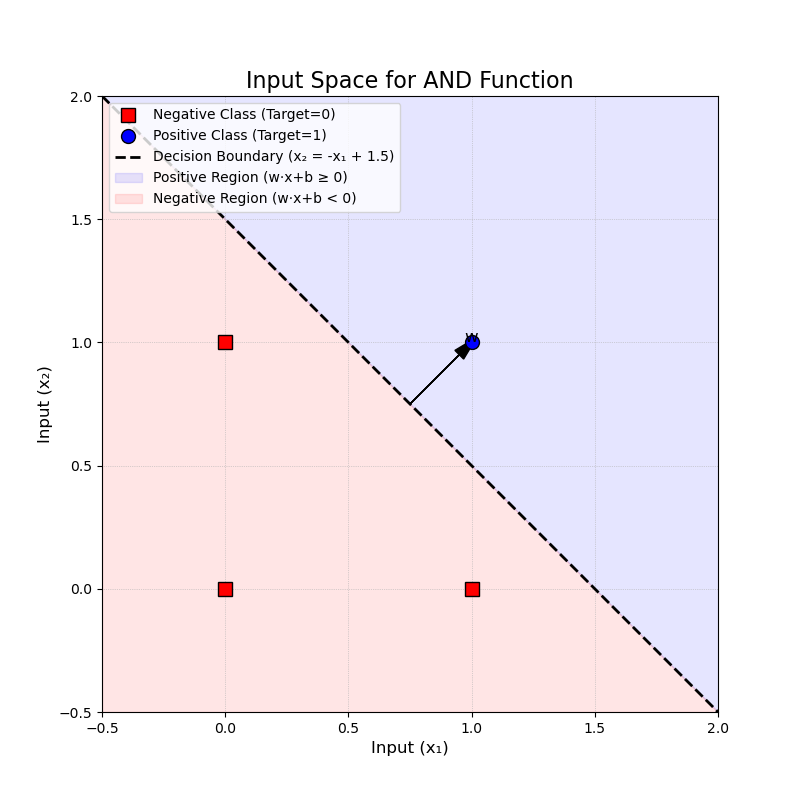
\includegraphics[width=0.6\textwidth]{and_input_space.png}
\caption{Input Space for the AND Function.}
\end{figure}

\subsubsection{The Weight Space}
The Weight Space represents the set of all possible solutions. Each of our four data points imposes a constraint on the possible values of the weights.
\begin{figure}[h!]
\centering
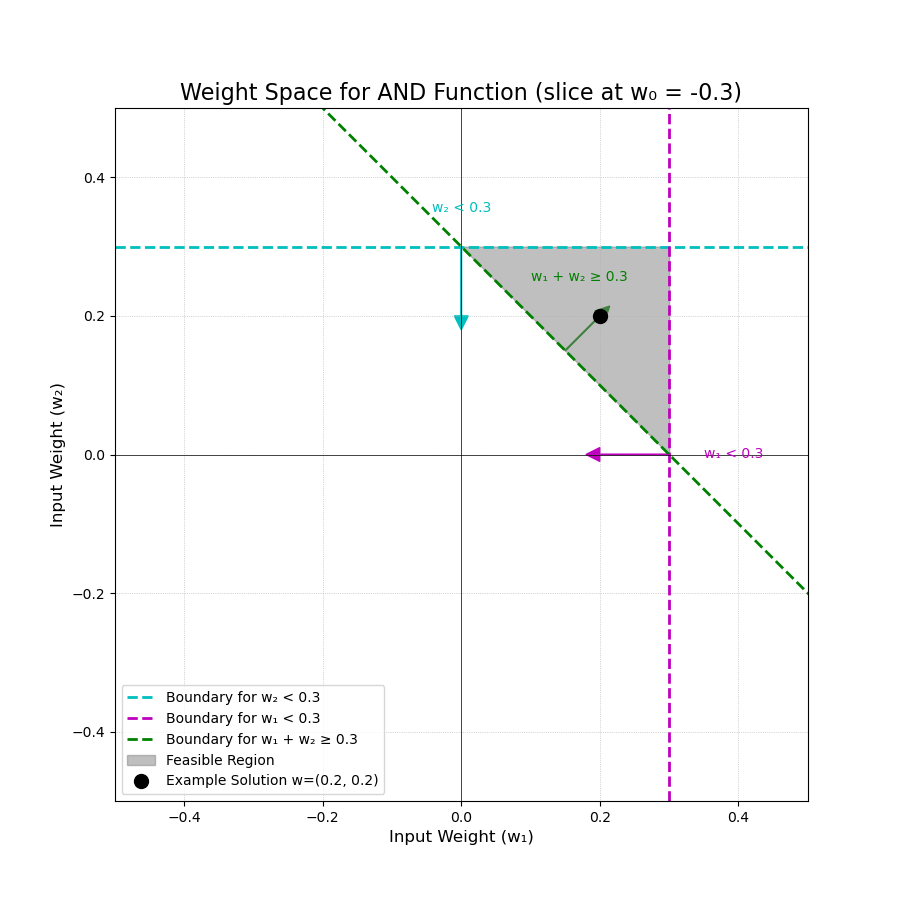
\includegraphics[width=0.6\textwidth]{and_weight_space.png}
\caption{A 2D slice of the Weight Space for the AND Function, with \(w_0 = -0.3\).}
\end{figure}

\section{Limitations of the Perceptron}
\subsection{Linear Separability Constraint}
The fundamental limitation of the perceptron is that it can only learn linearly separable functions.

\subsubsection{Definition: Linear Separability}
A dataset is \textbf{linearly separable} if there exists a hyperplane that perfectly separates the positive and negative examples:
\[\exists \mathbf{w}, b : y_i(\mathbf{w}^T \mathbf{x}_i + b) > 0 \quad \forall i\]

\subsubsection{The XOR Problem (Minsky \& Papert, 1969)}
Consider the XOR function:
\begin{center}
\begin{tabular}{|c|c|c|}
\hline
\(x_1\) & \(x_2\) & XOR \\
\hline
0 & 0 & 0 \\
0 & 1 & 1 \\
1 & 0 & 1 \\
1 & 1 & 0 \\
\hline
\end{tabular}
\end{center}

\textbf{Mathematical Proof of Non-Linear Separability}:
Assume there exists a linear classifier \(\mathbf{w}^T \mathbf{x} + b = 0\) that separates XOR data.
For the four points, we need:
\begin{align}
w_1 \cdot 0 + w_2 \cdot 0 + b &< 0 \quad \text{(point (0,0))} \\
w_1 \cdot 0 + w_2 \cdot 1 + b &> 0 \quad \text{(point (0,1))} \\
w_1 \cdot 1 + w_2 \cdot 0 + b &> 0 \quad \text{(point (1,0))} \\
w_1 \cdot 1 + w_2 \cdot 1 + b &< 0 \quad \text{(point (1,1))}
\end{align}

From equations (1) and (2): \(b < 0\) and \(w_2 + b > 0 \Rightarrow w_2 > -b > 0\)
From equations (1) and (3): \(b < 0\) and \(w_1 + b > 0 \Rightarrow w_1 > -b > 0\)
From equation (4): \(w_1 + w_2 + b < 0\)

But this contradicts \(w_1 > -b\) and \(w_2 > -b\), since:
\[w_1 + w_2 + b > -b + (-b) + b = -b > 0\]

Therefore, no linear separator exists for XOR.

\subsection{Solutions to Linear Separability Limitation}
\subsubsection{Multi-Layer Perceptrons (MLPs)}
\begin{itemize}
    \item Add hidden layers with non-linear activation functions
    \item Can approximate any continuous function (Universal Approximation Theorem)
    \item Require more sophisticated training algorithms (backpropagation)
\end{itemize}

\subsubsection{Feature Engineering}
\begin{itemize}
    \item Transform input space to make data linearly separable
    \item For XOR: Add feature \(x_3 = x_1 \oplus x_2\) (though this requires knowing the solution)
    \item Kernel methods: Implicitly map to higher-dimensional spaces
\end{itemize}

\subsubsection{Ensemble Methods}
\begin{itemize}
    \item Combine multiple linear classifiers
    \item Voting or weighted combination schemes
    \item Can learn non-linear decision boundaries
\end{itemize}

\section{Historical Impact and Legacy}
\subsection{The Perceptron Controversy}
The 1969 book "Perceptrons" by Minsky and Papert highlighted the limitations of single-layer perceptrons, leading to:
\begin{itemize}
    \item \textbf{AI Winter}: Reduced funding and interest in neural networks
    \item \textbf{Focus shift}: Emphasis moved to symbolic AI and expert systems
    \item \textbf{Delayed progress}: Multi-layer networks existed but lacked efficient training methods
\end{itemize}

\subsection{Modern Relevance}
Despite limitations, perceptrons remain important because:
\begin{itemize}
    \item \textbf{Building blocks}: Neurons in modern deep networks are perceptron variants
    \item \textbf{Theoretical foundation}: Understanding linear classifiers is crucial
    \item \textbf{Computational efficiency}: Still useful for linearly separable problems
    \item \textbf{Online learning}: Perceptron learning rule works in streaming settings
\end{itemize}

\section{Exercises} 
 
\begin{enumerate}
    \item Determine the weights of a network with 4 input and 2 output units using Perceptron learning law
\end{enumerate}
Input:
\(\begin{pmatrix} 1 & 1 & 0 & 0 \\ 1 & 0 & 0 & 1 \\ 0 & 0 & 1 & 1 \\ 0 & 1 & 1 & 0 \end{pmatrix}\)
Output:
\( \begin{pmatrix} 1& 1 & 1 & 0 & 0 \end{pmatrix} \)
